% Figure 5, narrow screens. Apply, check, then change one thing. Labels: LABELS.md, Figure 5.
% Same text and crimson focus as fig5-apply-flow.tex, stacked for a phone. Width matches fig1 narrow.
\def\eeprepfigure{1}
\providecommand{\eepstyledir}{../style}% repo: ../style
\input{\eepstyledir/circuitikz-preamble.tex}
% Colours, fonts, and text styles for the Get hired figures.
% Input after style/circuitikz-preamble.tex (in the repo: ../../style/circuitikz-preamble.tex).
% Define \eepdark before this file for the dark build. Same names as the resume figures,
% plus the rest of the navy palette. Crimson (eepaccent) marks one thing per figure.
\setmainfont{Newsreader}[
  BoldFont={Newsreader Bold},
  ItalicFont={Newsreader Italic},
  BoldItalicFont={Newsreader Bold Italic},
]
\usetikzlibrary{arrows.meta,calc,decorations.pathreplacing}
\ifdefined\eepdark
  \definecolor{eepink}{HTML}{ECEEF2}
  \definecolor{eeptext}{HTML}{D0D4DB}
  \definecolor{eepinktwo}{HTML}{A6AFBF}
  \definecolor{eepmute}{HTML}{8F95A0}
  \definecolor{eepsilver}{HTML}{76808F}
  \definecolor{eeprule}{HTML}{3B4352}
  \definecolor{eepwash}{HTML}{17243A}
  \definecolor{eepsunken}{HTML}{101828}
  \definecolor{eepfill}{HTML}{131C2E}
  \definecolor{eeppaper}{HTML}{0D1524}
  \definecolor{eepaccent}{HTML}{E06A5F}
  \definecolor{eepaccentsoft}{HTML}{2A1A24}
\else
  \definecolor{eepink}{HTML}{16233A}
  \definecolor{eeptext}{HTML}{232A39}
  \definecolor{eepinktwo}{HTML}{424D63}
  \definecolor{eepmute}{HTML}{5E636C}
  \definecolor{eepsilver}{HTML}{838C9A}
  \definecolor{eeprule}{HTML}{C4C8CF}
  \definecolor{eepwash}{HTML}{E7ECF3}
  \definecolor{eepsunken}{HTML}{F3F4F6}
  \definecolor{eepfill}{HTML}{FFFFFF}
  \definecolor{eeppaper}{HTML}{FBFBFC}
  \definecolor{eepaccent}{HTML}{A3201D}
  \definecolor{eepaccentsoft}{HTML}{F8ECEA}
\fi
% Draw in y-down points so coordinates read like a mockup: [x=1pt, y=-1pt].
\tikzset{
  eeptitle/.style={anchor=base west, inner sep=0pt, text=eepink, font=\rmfamily\bfseries\fontsize{26}{31}\selectfont},
  eephead/.style={inner sep=0pt, text=eepink, font=\sffamily\bfseries\fontsize{14.5}{18}\selectfont},
  eepbody/.style={inner sep=0pt, text=eepinktwo, font=\sffamily\fontsize{13}{17}\selectfont},
  eepnote/.style={inner sep=0pt, text=eepmute, font=\sffamily\fontsize{12.5}{16}\selectfont},
  eepsrc/.style={anchor=north west, inner sep=0pt, align=left, text=eepmute, font=\sffamily\fontsize{11}{14.5}\selectfont},
  eepbox/.style={draw=eepink, fill=eepfill, rounded corners=4pt},
  eepfocus/.style={draw=eepaccent, fill=eepfill, rounded corners=4pt, line width=1.8pt},
  eeparrow/.style={-{Stealth[length=8pt,width=6pt]}},
  eepdash/.style={dash pattern=on 4pt off 4pt},
  eeplead/.style={draw=eepsilver, line width=0.9pt},
}
% A dot on a trace, like a schematic junction.
\newcommand{\eepdot}[2][eepink]{\fill[#1] #2 circle (3.6pt);}
% Short labels never hyphenate.
\hyphenpenalty=10000 \exhyphenpenalty=10000
% One space after a full stop, as on the site.
\frenchspacing

% #1 x1, #2 y1, #3 x2, #4 y2, #5 style, #6 text
\newcommand{\flowbox}[6]{%
  \draw[#5] (#1,#2) rectangle (#3,#4);
  \node[eephead, align=center, text width={#3-#1-24}] at ({(#1+#3)/2},{(#2+#4)/2}) {#6};}
\begin{document}
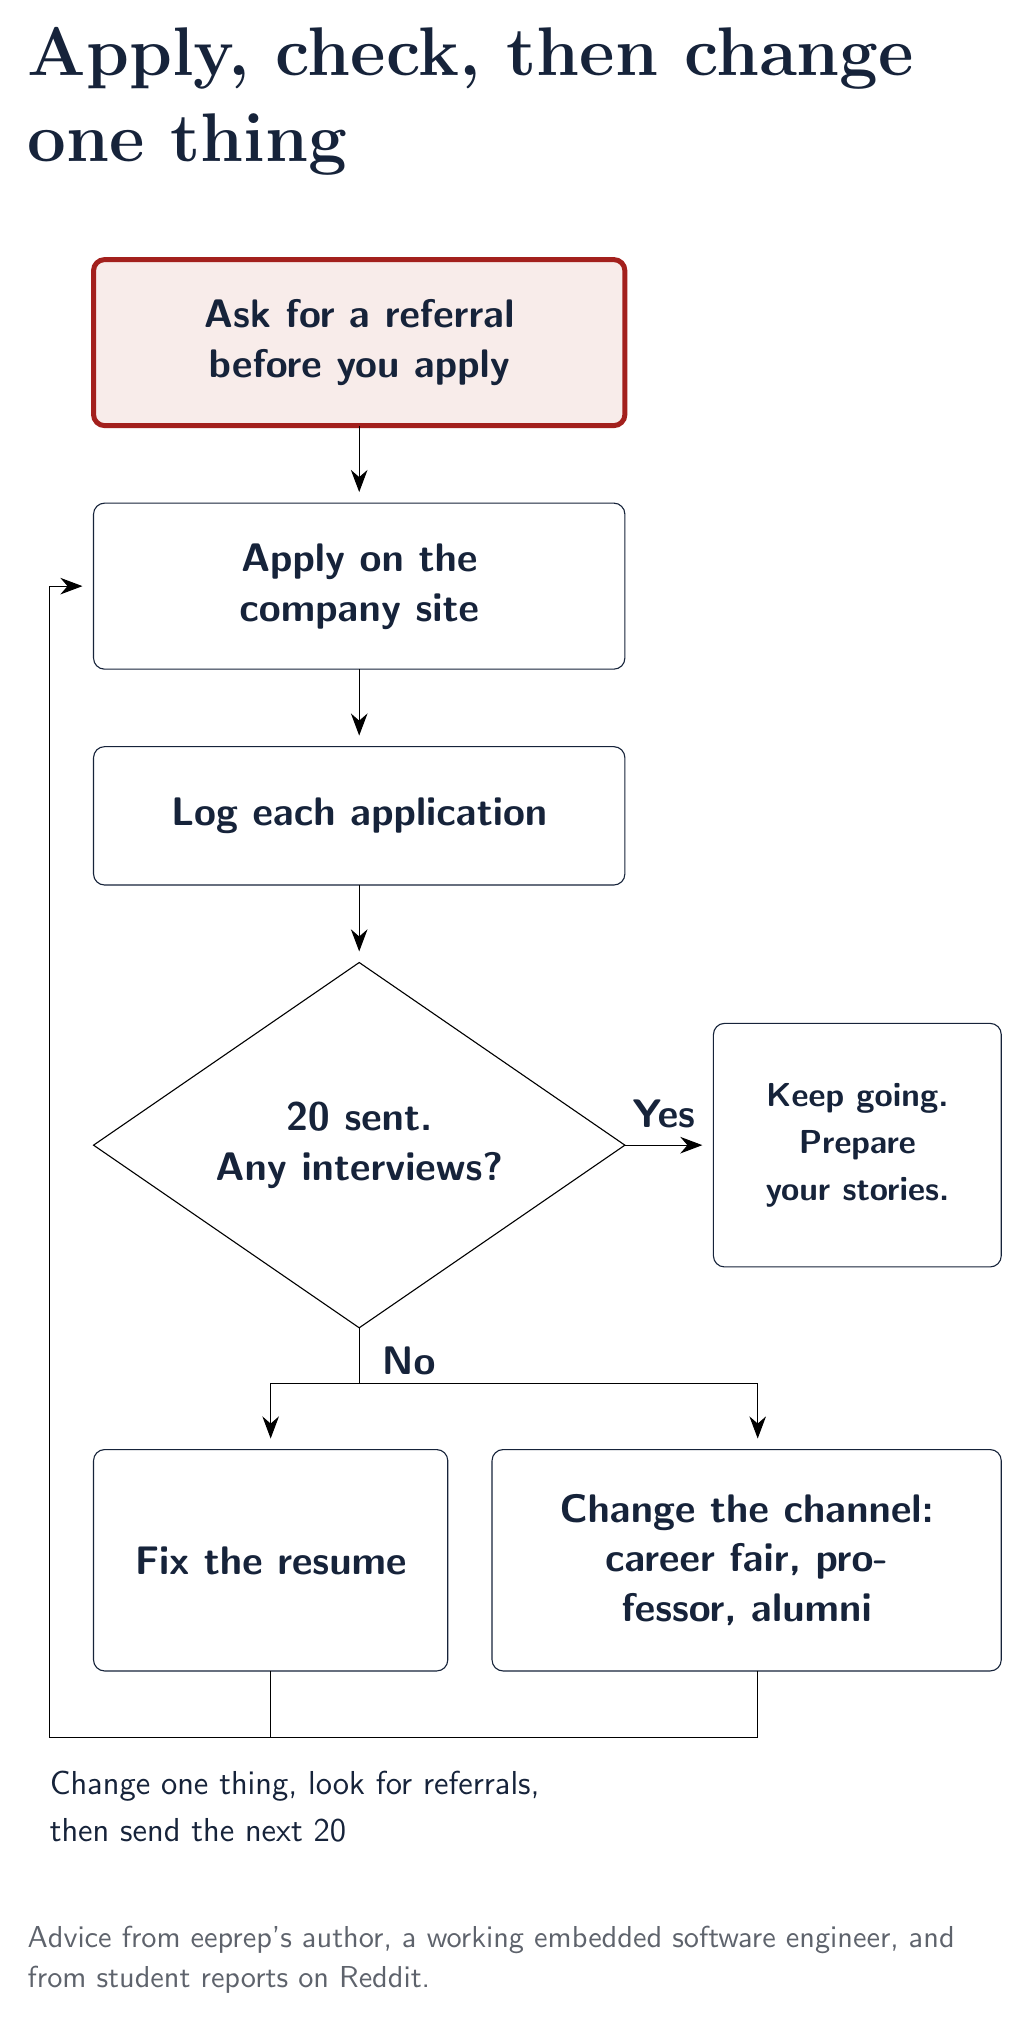
\begin{tikzpicture}[x=1pt,y=-1pt]
  \node[eeptitle, anchor=north west, text width=354pt, align=left] at (0,4) {Apply, check, then change one thing};
  % Main column, centre x = 120.
  \flowbox{24}{88}{216}{148}{eepfocus, fill=eepaccentsoft}{Ask for a referral before you apply}
  \draw[eeparrow] (120,148) -- (120,172);
  \flowbox{24}{176}{216}{236}{eepbox}{Apply on the company site}
  \draw[eeparrow] (120,236) -- (120,260);
  \flowbox{24}{264}{216}{314}{eepbox}{Log each application}
  \draw[eeparrow] (120,314) -- (120,338);
  \draw[fill=eepfill, line join=miter] (120,342) -- (216,408) -- (120,474) -- (24,408) -- cycle;
  \node[eephead, align=center, text width=110pt] at (120,408) {20 sent.\\ Any interviews?};
  % Yes: to the right.
  \draw[eeparrow] (216,408) -- (244,408);
  \node[eephead, anchor=south] at (230,402) {Yes};
  \draw[eepbox] (248,364) rectangle (352,452);
  \node[eephead, align=center, text width=96pt, font=\sffamily\bfseries\fontsize{13}{17}\selectfont] at (300,408) {Keep going.\\ Prepare\\ your stories.};
  % No: down to the two options, side by side.
  \draw (120,474) -- (120,494);
  \node[eephead, anchor=west] at (128,486) {No};
  \draw (88,494) -- (264,494);
  \draw[eeparrow] (88,494) -- (88,514);
  \draw[eeparrow] (264,494) -- (264,514);
  \flowbox{24}{518}{152}{598}{eepbox}{Fix the resume}
  \flowbox{168}{518}{352}{598}{eepbox}{Change the channel:\\ career fair, professor, alumni}
  % The loop back to Box 1, up the left edge.
  \draw (88,598) -- (88,622);
  \draw (264,598) -- (264,622) -- (8,622) -- (8,206);
  \draw[eeparrow] (8,206) -- (20,206);
  \node[eepbody, text=eepink, anchor=north west, text width=346pt, align=left] at (8,634) {Change one thing, look for referrals,\\ then send the next 20};
  \node[eepsrc, text width=354pt] at (0,690) {Advice from eeprep's author, a working embedded software engineer, and from student reports on Reddit.};
\end{tikzpicture}
\end{document}
